\subsection*{Esercizio 10.2 Hoff} % (fold)

Nesting success: younger male sparrows may or may not nest during a mating season, perhaps depending on their physical characteristics. Researchers have recorded the nesting success of 43 young male sparrows of the same age, as well as their wingspan, and the data appear in the file \texttt{msparrownest.dat}. Let $Y_i$ be the binary indicator that sparrow $i$ successfully nests, and let $x_i$ denote their wingspan. Our model for $Y_i$ is $logit\theta(Y_i = 1|\alpha, \beta, x_i)) = \alpha + \beta x_i$, where the logit function is given by $logit \theta = log\left[\frac{\theta}{1-\theta}\right]$.
\begin{enumerate}
  \item Write out the joint sampling distribution  $\prod_{i=1}^{n}p(y_i | \alpha, \beta, x_i)$ and simplify as much as possible.
  \item Formulate a prior probability distribution over $\alpha$ and $\beta$ by considering the range of $Pr(Y = 1|\alpha,\beta,x)$ as x ranges over $10$ to $15$, the approximate range of the observed wingspans.
  \item Implement a Metropolis algorithm that approximates $p(\alpha, \beta|\mathbf{y}, \mathbf{x})$. Adjust the proposal distribution to achieve a reasonable acceptance rate, and run the algorithm long enough so that the effective sample size is at least $1,000$ for each parameter.
  \item Compare the posterior densities of $\alpha$ and $\beta$ to their prior densities.
  \item Using output from the Metropolis algorithm, come up with a way to make a confidence band for the following function $f_{\alpha\beta}(x)$ of wingspan:
  $$f_{\alpha\beta}(x) = \frac{e^{\alpha + \beta x}}{1+e^{\alpha + \beta x}}$$
  where $\alpha$ and $\beta$ are the parameters in your sampling model. Make a plot of such a band.
\end{enumerate}


\textbf{Svolgimento}:
\bigskip

L'esercizio ha come obiettivo principale quello di studiare la relazione tra la probabilità di nidificare e l'ampiezza delle ali per un gruppo di $43$ uccellini maschi della stessa età. 
Il setting del modello è il seguente:
$$Y_i = \begin{cases} 1, & \mbox{se l'uccellino } i\mbox{ nidifica} \\ 0, & \mbox{altrimenti } \end{cases}; \quad x_i = \text{ampiezza dell'uccellino } i; \quad i = 1, \dots, 43$$
La verosomiglianza per ogni singola osservazione è pertanto una Bernoulli:
$$p(y_i | p_i) = p_i^{y_i}(1-p_i)^{1-y_i}$$
Studiamo la relazione tra la probabilità di nidificare e l'ampiezza delle ali con il modello logistico (siamo quindi nell'ambito dei modelli lineari generalizzati):
$$g(p_i) = logit(p_i) = log\left(\frac{p_i}{1-p_i}\right) = \eta_i = \alpha + \beta x_i$$
pertanto
$$g^{-1}(\eta_i) = p_i = \frac{e^{\eta_i}}{1+e^{\eta_i}} = \frac{e^{\alpha + \beta x_i}}{1+e^{\alpha + \beta x_i}}$$
\subsubsection*{Parte a} 
Scriviamo la verosomiglianza secondo il modello appena descritto, quindi come funzione di $\alpha$ e $\beta$ (ricordiamo l'indipendenza condizionata a tali parametri):
\begin{gather}
\nonumber\mathcal{L}(\alpha;\beta;\mathbf{y};\mathbf{X}) = p(\mathbf{y}|\alpha, \beta, \mathbf{X}) = \prod_{i=1}^{n}p(y_i |\alpha, \beta, \mathbf{x_i}) = \prod_{i=1}^{n}\left[\left(\frac{e^{\eta_i}}{1+e^{\eta_i}}\right)^{y_i}\left(\frac{1}{1+e^{\eta_i}}\right)^{1-y_i}\right] \\
\nonumber=\prod_{i=1}^{n} \frac{e^{y_i\eta_i}}{1+e^{\eta_i}} = \prod_{i=1}^{n}(e^{y_i\eta_i} - log(1-e^{\eta_i})) = e^{\sum_{i=1}^{n}[y_i\eta_i - log(1+e^{\eta_i})]} \\
\nonumber=e^{\sum_{i=1}^{n}[y_i(\alpha+\beta x_i) - log(1+e^{\alpha+\beta x_i})]}
\end{gather}
Potevamo in maniera analoga procedere passando direttamente attraverso la scrittura delle singole verosomiglianze nella forma della famiglia esponenziale in questo modo:
$$p(y_i|p_i) = p_i^{y_i}(1-p_i)^{1-y_i} = e^{y_i log(\frac{p_i}{1-p_i}+log(1-p_i))}$$
quindi
\begin{gather}
\nonumber \prod_{i=1}^{n} p(y_i|p_i) = \prod_{i=1}^{n} e^{\sum_{i=1}^{n}[y_i \eta_i + log(\frac{1}{1+\eta_i})]} = e^{\sum_{i=1}^{n}[y_i \eta_i + log(1+\eta_i)]}\\
\nonumber e^{\sum_{i=1}^{n}[y_i(\alpha+\beta x_i) - log(1+e^{\alpha+\beta x_i})]}
\end{gather}
\subsubsection*{Parte b} % (fold)
Possiamo formulare la a priori per $\alpha$ e $\beta$ nei seguenti modi:
\begin{enumerate}
  \item \textbf{soggettivamente:} a priori pensiamo che la probabilità di nidificare sia alta e che vari tra $[0.5, 0.9]$; sapendo inoltre che il campo di variazione della covariata è $[10, 15]$, troviamo il range di $\alpha$ e $\beta$ che sia compatibile con quello della probabilità e in base ad esso formuliamo la prior sui parametri. In dettaglio: Pensiamo che $p=Pr(Y=1 | \alpha, \beta, \mathbf{x}) \in [0.5, 0.9]$ e quindi che $logit(p) = log\left(\frac{p}{1-p}\right) = \alpha + \beta x \in [0, 2.2]$. Si ha il seguente sistema di disequazioni:
  $$\begin{cases} \alpha+\beta x \geq 0 \\ \alpha + \beta x \leq 2.2 \end{cases}$$
  Troviamo il range di $\alpha$ e di $\beta$ risolvendo il sistema per il valore minimo e per quello massimo di x:
  $$\begin{cases} \alpha+10\beta = 0 \\ \alpha +  15\beta = 2.2 \end{cases} \begin{cases}\beta = 0.44 \\ \alpha = -4.4\end{cases} \begin{cases} \alpha+15\beta = 0 \\ \alpha +  10\beta = 2.2 \end{cases} \begin{cases}\beta = -0.44 \\ \alpha = -4.4\end{cases}$$
  Quindi $\beta \in [-0.44, 0.44]$ e $\alpha \in [-4.4 6.6]$.
  Specifichiamo come vettore delle medie il centroide $(\alpha_0, \beta_o)^T$ = $(1.1, 0)^T$.
  Resta da specificare la matrice di varianza e covarianza. Innanzitutto, dal momento che i valori di $\alpha$ e $\beta$ che sono contemporaneamente massimi e contemporanea\-mente minimi generano valori del logit fuori dal range a priori, prendiamo covarianza nulla tra i due parametri in modo che i valori appena citati siano meno probabili: $\sigma_{\alpha\beta} = 0$. Per specificare le varianze $\sigma_{\alpha}^2$ e $\sigma_{\beta}^2$ seguiamo la logica degli intervalli di confidenza: date le distribuzioni normali di $\alpha$ e $\beta$, sappiamo che:
  $$P(\alpha_0 - 2\sigma_\alpha \leq x \leq \alpha_0 + 2\sigma_\alpha) \simeq 0.95; \qquad P(\beta_0 - 2\sigma_\beta \leq x \leq \beta_0 + 2\sigma_\beta) \simeq 0.95$$
  Quindi cerchiamo le deviazioni standard in modo che
  $$2\sigma_\alpha =  \frac{6.6 - (-4.4)}{2} = 5.5; \qquad 2\sigma_\beta = 0.44$$
  e si ha che
  $$\sigma_\alpha 2.75; \qquad \sigma_beta = 0.22$$
  Per tutto quanto detto, la prior formulata considerando il range di $P(Y=1 | \alpha, \beta, x)$ al variare di $x$ in $[10, 15]$ è:
  $$\binom{\alpha}{\beta} \sim N_2\left(\binom{\alpha_0}{\beta_0},
  \begin{pmatrix}
    \sigma^2_\alpha & \sigma^2_{\alpha\beta} \\
    \sigma^2_{\alpha\beta} & \sigma^2_\beta

  \end{pmatrix}\right) \equiv N_2 \left(\binom{1.1}{0} \begin{pmatrix} 2.75^2 & 0 \\ 0 & 0.22^2 \end{pmatrix}\right)$$
\end{enumerate}
Rispondiamo adesso alle altre richieste dell'esercizio in R.

\begin{lstlisting}[style=R]
#Funzione per campionare da una distribuzione normale multivariata
rmvnorm <- function(n, mu, Sigma)
{
  #samples form the multivariate normal distribution
  E<-matrix(rnorm(n*length(mu)), n, length(mu))
  t( t(E%*%chol(Sigma)) +c(mu))
}
#Lettura dei dati :
dati<-as.matrix(dati<-read.table(
  "/home/mameli/git/notebookInferenzaBayesiana/code/msparrownest.dat", 
  col.names=c("Y" , "X")))
\end{lstlisting}

{
\color{red}
\begin{Verbatim}
> head(dati)
      Y       X 
[1,]  0     13.03 
[2,]  1     13.69 
[3,]  1     12.62 	
[4,]  0     11.70 	
[5,]  0     12.39 	
[6,]  0     12.44
\end{Verbatim}
}

\begin{lstlisting}[style=R]
#Matrice del modello e vettore delle osservazioni :
X = cbind(1, dati[,2])
\end{lstlisting}

{
\color{red}
\begin{Verbatim}
> head(X)
    [,1]    [,2]
[1,]  1     13.03
[2,]  1     13.69
[3,]  1     12.62
[4,]  1     11.70
[5,]  1     12.39
[6,]  1     12.44
\end{Verbatim}
}

\begin{lstlisting}[style=R]
y = dati[,1]
\end{lstlisting}

{
\color{red}
\begin{Verbatim}
> head(y)
[1] 0 1 1 0 0 0
\end{Verbatim}
}

\begin{lstlisting}[style=R]
n<-length(y)
p<-dim(X)[2]

#b) inizializziamo la prior:

pmn.beta<-c(1.1, 0)
psd.beta<-c(2.75, 0.22)

library(coda)
metropolis<-function(tuning, nsimul) {	
  pmn.beta<-c(1.1, 0)
  psd.beta<-c(2.75, 0.22)
  var.prop<-tuning
  beta<-rep(0, p)
  S<-nsimul
  BETA<-matrix(0, nrow=S, ncol=p)
  ac<-0
  set.seed(1)
  for(s in 1:S){
    beta.p<-t(rmvnorm(1, beta, var.prop))
    lhr<- sum(log(dbinom(y,1,exp(X%*%beta.p)/(1+exp(X%*%beta.p))))) + dnorm(beta.p[1],pmn.beta[1],psd.beta[1],log=TRUE) + dnorm(beta.p[2],pmn.beta[2],psd.beta[2],log=TRUE)-sum(log(dbinom(y,1,exp(X%*%beta)/(1+exp(X%*%beta)))))-dnorm(beta[1],pmn.beta[1],psd.beta[1],log=TRUE)-dnorm(beta[2],pmn.beta[2],psd.beta[2],log=TRUE)
    if(log(runif(1))<lhr) beta<-beta.p; ac<-ac+1
    BETA[s,]<-beta 
  }
  Ef<-effectiveSize(BETA)
  
  cat("acceptance rate=", ac/S, "\n")
  cat("effective sample size=", Ef, "\n")
  return (BETA)
}
eturn (BETA)
}
nsimul <- 1000
var.prop <- var(log(y + 1 / 2)) * solve(t(X) %*% X)
\end{lstlisting}

{
\color{red}
\begin{Verbatim}
> var.prop
            [,1]		[,2]
[1,]  1.11413865	-0.085406852
[2,]  -0.085406852	0.006588971
\end{Verbatim}
}

\begin{lstlisting}[style=R]
beta.post <- metropolis(var.prop, nsimul)
\end{lstlisting}

{
\color{red}
\begin{Verbatim}
Acceptance rate = 0.764
Effective sample size = 51.65653
\end{Verbatim}
}

\begin{lstlisting}[style=R]
  var.prop <- var.prop*9
  nsimul <- 5000
  beta.post <- metropolis( var.prop, nsimul)
\end{lstlisting}
  
{\color{red}
\begin{verbatim}
acceptance rate= 1 
effective sample size= 915.514 912.21 
\end{verbatim}
}

\begin{lstlisting}[style=R]
  skips<-seq(5,nsimul,by=10)
  plot(skips ,beta.post[skips ,1], type="l", xlab="iteration",ylab=expression(alpha), col = "red")
  plot(skips, beta.post[skips ,2] ,type="l",xlab="iteration", ylab=expression (beta), col = "blue")
\end{lstlisting}
  
\begin{figure}[htbp]
  \label{fig:grafici}
  \centering
  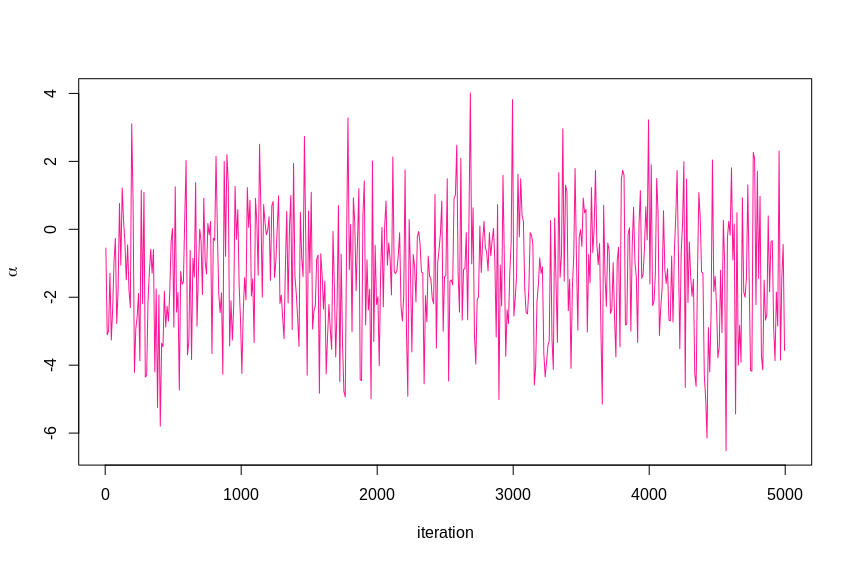
\includegraphics[width=0.8\linewidth]{img/esercizio10-2-1}% "%" necessario
  \qquad\qquad
  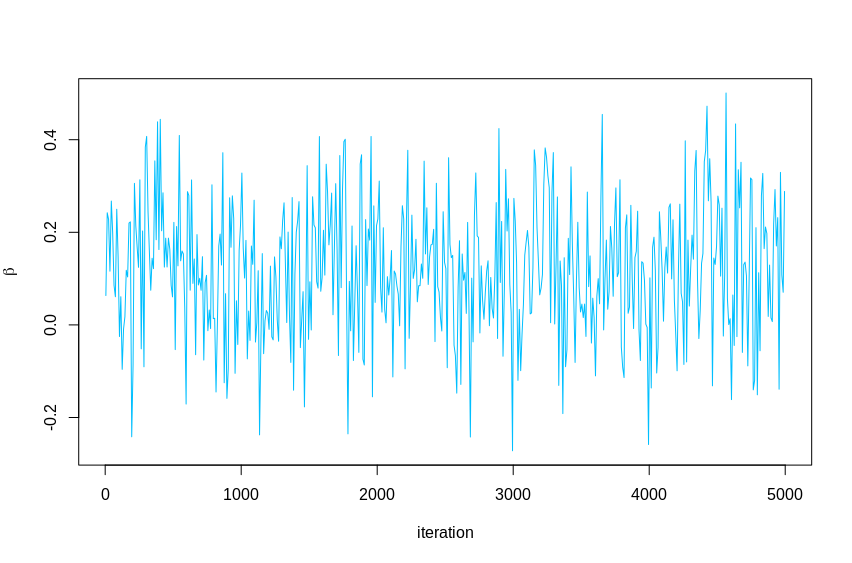
\includegraphics[width=0.8\linewidth]{img/esercizio10-2-2}
\end{figure}

Facciamo adesso il confronto delle distribuzioni a priori e posteriori dei coeffi\-cienti di regressione:

\begin{lstlisting}[style=R]
par(mfrow=c(1,2))
x<-seq(-10, 10, by=0.1)
plot(x, dnorm(x, pmn.beta[1], psd.beta[1]) ,ylim=c(0,0.25), type="l",lwd=1, xlab=expression(alpha), ylab="density", col = "orange")
lines(density(beta.post[ ,1]) , col = "red")
legend("topright",legend=c("Prior","Posterior"),lty = c(1,1),cex=0.7, bty="n",seg.len=1.5,  col = c("orange","red"))
y<-seq(-2,2,by=0.01)
plot(y,dnorm(y,pmn.beta[2],psd.beta[2]), ylim=c(0,3), type="l", lwd=1, xlab=expression(beta), ylab="density", col = "orange")
lines(density(beta.post[ ,2]) , col="red")
legend("topright",legend=c("Prior","Posterior"),lty = c(1,1),cex=0.7,bty="n", seg.len=1.5, col = c("orange","red"))
\end{lstlisting}
\begin{figure}[h!]
  \centering
  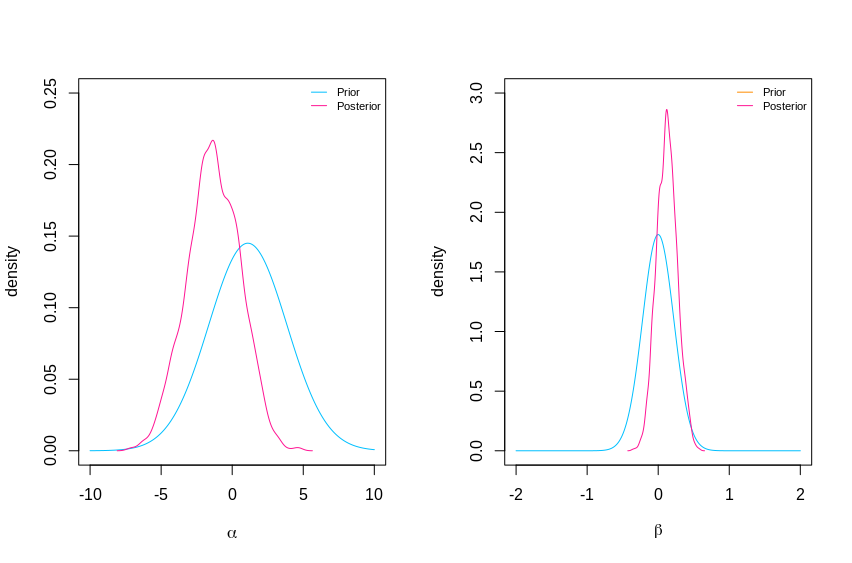
\includegraphics[width=0.7\linewidth]{img/esercizio10-2-3}
  \label{fig:metropolis3}
\end{figure}

\begin{lstlisting}[style = R]
  f<-exp(t(X%*%t(beta.post)))/(1+exp(t(X%*%t(beta.post))))
  qE<-apply(f,2,quantile,probs=c(0.025,0.975))
  par(mfrow=c(1,1))
  plot(c(10,15),range(c(0,qE)),type="n",xlab="wingspan",ylab="f")
  lines(qE[1,],col="deepskyblue",lwd=2)
  lines(qE[2,],col="deeppink",lwd=2)
\end{lstlisting}
Notiamo che la distribuzione a posteriori dà probabilità maggiore a valori più bassi di $\alpha$ e a valori più alti di $\beta$ rispetto a quella a priori. 
Questo significa che avevamo ipotizzato una proabilità di nidificare un po' troppo alta.

Approssimiamo adesso la funzione richiesta nel punto e, utilizzando i risultati dell'algoritmo di Metropolis. Tracciamo anche la banda di confidenza al $95\%$.
\begin{figure}[h!]
  \centering
  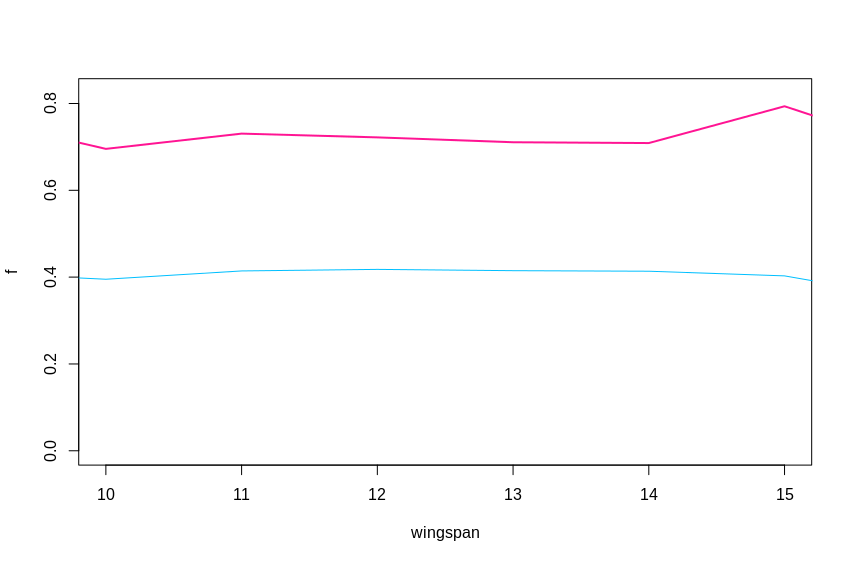
\includegraphics[width=0.7\linewidth]{img/esercizio10-2-4}
  \label{fig:metropolis4}
\end{figure}

Dal grafico si evince che l'ampiezza delle ali non influenza la probabilità di nidificare poichè la banda di confidenza è praticamente parallela all'asse delle ascisse.

